%%%%%%%%%%%%%%%%%%%%%%%%%%%%%%%%%%%%%%%%%
% Beamer Presentation
% LaTeX Template
% Version 1.0 (10/11/12)
%
% This template has been downloaded from:
% http://www.LaTeXTemplates.com
%
% License:
% CC BY-NC-SA 3.0 (http://creativecommons.org/licenses/by-nc-sa/3.0/)
%
%%%%%%%%%%%%%%%%%%%%%%%%%%%%%%%%%%%%%%%%%

%----------------------------------------------------------------------------------------
%	PACKAGES AND THEMES
%----------------------------------------------------------------------------------------

\documentclass{beamer}

\mode<presentation> {

% The Beamer class comes with a number of default slide themes
% which change the colors and layouts of slides. Below this is a list
% of all the themes, uncomment each in turn to see what they look like.

%\usetheme{default}
%\usetheme{AnnArbor}
%\usetheme{Antibes}
%\usetheme{Bergen}
%\usetheme{Berkeley}
%\usetheme{Berlin}
%\usetheme{Boadilla}
%\usetheme{CambridgeUS}
%\usetheme{Copenhagen}
%\usetheme{Darmstadt}
%\usetheme{Dresden}
%\usetheme{Frankfurt}
%\usetheme{Goettingen}
%\usetheme{Hannover}
%\usetheme{Ilmenau}
%\usetheme{JuanLesPins}
%\usetheme{Luebeck}
\usetheme{Madrid}
%\usetheme{Malmoe}
%\usetheme{Marburg}
%\usetheme{Montpellier}
%\usetheme{PaloAlto}
%\usetheme{Pittsburgh}
%\usetheme{Rochester}
%\usetheme{Singapore}
%\usetheme{Szeged}
%\usetheme{Warsaw}

% As well as themes, the Beamer class has a number of color themes
% for any slide theme. Uncomment each of these in turn to see how it
% changes the colors of your current slide theme.

%\usecolortheme{albatross}
%\usecolortheme{beaver}
%\usecolortheme{beetle}
%\usecolortheme{crane}
%\usecolortheme{dolphin}
%\usecolortheme{dove}
%\usecolortheme{fly}
%\usecolortheme{lily}
%\usecolortheme{orchid}
%\usecolortheme{rose}
%\usecolortheme{seagull}
%\usecolortheme{seahorse}
%\usecolortheme{whale}
%\usecolortheme{wolverine}

%\setbeamertemplate{footline} % To remove the footer line in all slides uncomment this line
%\setbeamertemplate{footline}[page number] % To replace the footer line in all slides with a simple slide count uncomment this line

%\setbeamertemplate{navigation symbols}{} % To remove the navigation symbols from the bottom of all slides uncomment this line
}

\usepackage{graphicx} % Allows including images
\usepackage{booktabs} % Allows the use of \toprule, \midrule and \bottomrule in tables

%----------------------------------------------------------------------------------------
%	TITLE PAGE
%----------------------------------------------------------------------------------------

\title[Signal Processing on Graphs]{Journal Club: The Emerging Field of Signal Processing on Graphs} % The short title appears at the bottom of every slide, the full title is only on the title page

\author{Matt Bartos} % Your name
\institute[UM] % Your institution as it will appear on the bottom of every slide, may be shorthand to save space
{
University of Michigan \\ % Your institution for the title page
\medskip
\textit{mdbartos@umich.edu} % Your email address
}
\date{\today} % Date, can be changed to a custom date

\begin{document}

\begin{frame}
\titlepage % Print the title page as the first slide
\end{frame}

\begin{frame}
\frametitle{Overview} % Table of contents slide, comment this block out to remove it
\tableofcontents % Throughout your presentation, if you choose to use \section{} and \subsection{} commands, these will automatically be printed on this slide as an overview of your presentation
\end{frame}

%----------------------------------------------------------------------------------------
%	PRESENTATION SLIDES
%----------------------------------------------------------------------------------------

%------------------------------------------------
\section{Other work on graph signals} % Sections can be created in order to organize your presentation into discrete blocks, all sections and subsections are automatically printed in the table of contents as an overview of the talk
%------------------------------------------------

\begin{frame}
\frametitle{Other work on graph signals}

\begin{description}
\item[\textbf{SNFOV}] Shuman, D. I., Narang, S. K., Frossard, P., Ortega, A., \&
  Vandergheynst, P. (2013). The emerging field of signal processing on graphs:
  Extending high-dimensional data analysis to networks and other irregular
  domains. Signal Processing Magazine, IEEE, 30(3), 83-98.

\item[ZFC] Zhang, C., Florencio, D., \& Chou, P. A. (2015). Graph signal processing: a
  probabilistic framework. Microsoft Res., Redmond, WA, USA, Tech. Rep.
  MSR-TR-2015-31.

\item[MSLR] Marques, A. G., Segarra, S., Leus, G., \& Ribeiro, A. (2016). Sampling of
  graph signals with successive local aggregations. IEEE Transactions on Signal
  Processing, 64(7), 1832-1843.

\item[PV] Perraudin, N., \& Vandergheynst, P. (2017). Stationary signal processing on
  graphs. IEEE Transactions on Signal Processing, 65(13), 3462-3477.
\end{description}
\end{frame}

%------------------------------------------------
\section{Contribution of Shuman et al.}
%------------------------------------------------

\begin{frame}
  \frametitle{Contribution of Shuman et al.}
  This is a tutorial review paper:
  
  \begin{itemize}
  \item Reviews existing work
  \item Provides definitions for graph signal operations and transforms (e.g. graph
    signal translation, graph Fourier transform)
  \item Provides example implementations (e.g. Tikhonov regularization, wavelet filtering)
  \item Summarizes open issues in the field
  \end{itemize}
\end{frame}

\begin{frame}
  \frametitle{Topics}
  \begin{itemize}
  \item Challenges of signal processing on graphs
  \item The Graph Laplacian
  \item Definition of the Graph Fourier transform
  \item Metrics of signal smoothness
  \item Generalized operators for signals on graphs
    \begin{itemize}
    \item Filtering
    \item Translation
    \item Convolution
    \item Modulation and Dilation
    \end{itemize}
  \item Graph coarsening
  \item Graph wavelet filtering
  \end{itemize}
\end{frame}


\begin{frame}
  \frametitle{Challenges of graph signal processing}
  How can we extend traditional signal processing tools to graphs?
  \begin{itemize}
    \item Translation, downsampling and modulation of signals in the graph
      domain
    \item How to implement filtering operations on graphs
  \end{itemize}

  Challenges:
  \begin{itemize}
  \item Graphs are irregular structures that lack a shift-invariant notion of translation.
  \item Modulation is nontrivial, given that the graph frequency spectrum is
    discrete and irregularly spaced.
  \item Downsampling is nontrivial, as there is no notion of ``every other
    vertex''.
  \item How can we capture the structure of the graph in downsampling operations?
  \end{itemize}
\end{frame}

%------------------------------------------------

\begin{frame}
\frametitle{Review of the Fourier Transform}

In the traditional Euclidean domain, we can find the frequency-domain
representation of a time series signal using the Fourier transform:

\begin{block}{Classical Fourier Transform}
  \begin{equation}
    \hat{f}(\xi) = \int_{-\infty}^{\infty} f(t) e^{-2 \pi j \xi t} dt 
  \end{equation}
\end{block}

$\hat{f}$ is an expansion of $f$ in terms of complex exponentials, which are the
eigenfunctions of the Laplace operator:

\begin{block}{Classical Fourier transform in terms of the Laplace operator}
  \begin{equation}
    - \Delta (e^{2 \pi j \xi t}) = - \frac{\partial^2}{\partial t^2} e^{2 \pi j \xi t} = 4 \pi^2 \xi^2 e^{2 \pi j \xi t} = k e^{2 \pi j \xi t}
  \end{equation}
\end{block}
\end{frame}

\begin{frame}  
  \frametitle{Classical Fourier Transform}
\begin{figure}
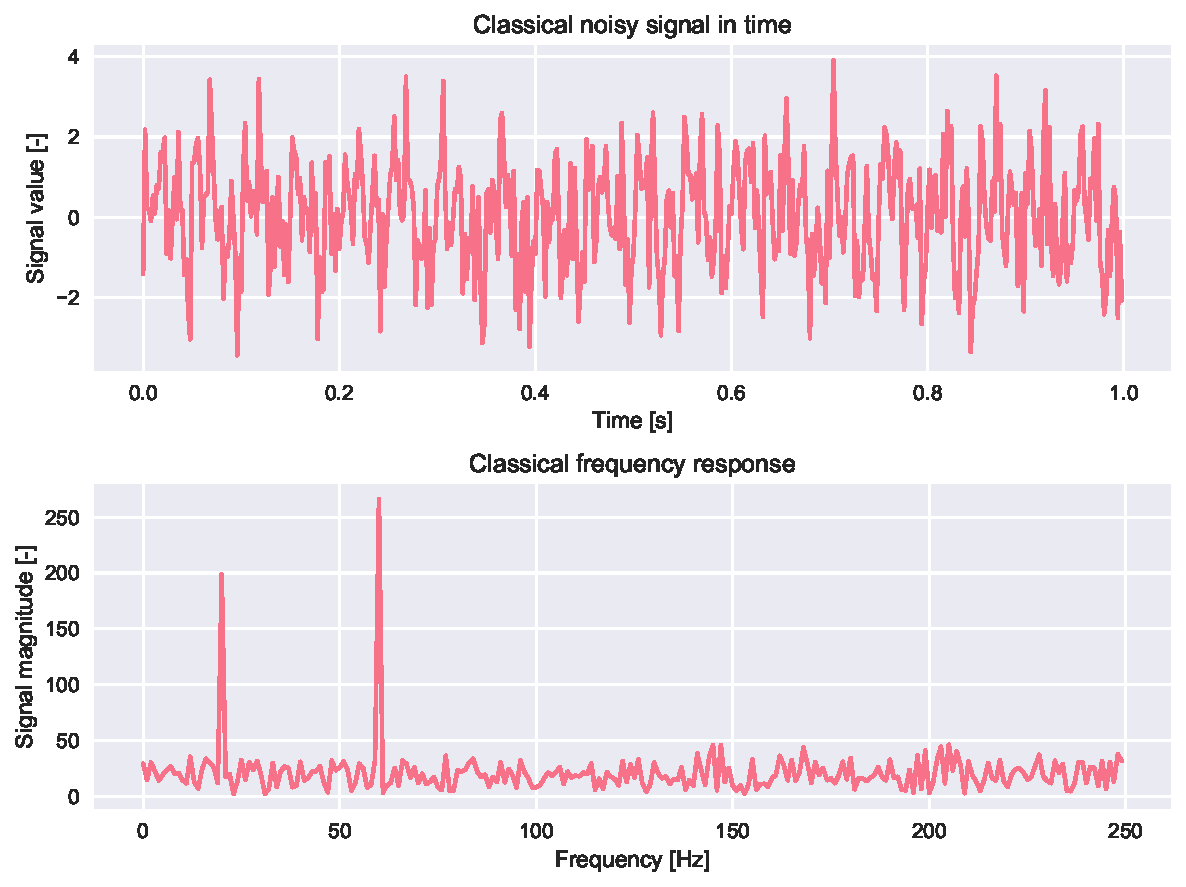
\includegraphics[width=0.7\linewidth]{../img/graph_fourier_transform_0.pdf}
\end{figure}
\end{frame}


\begin{frame}
\frametitle{The Graph Laplacian}

For each vertex $i$, the Laplace operator computes the weighted sum of the
differences between the signal value at $i$ and the signal value at $i's$
neighbors ($j \in N_i$). 

\begin{block}{The Laplacian is a difference operator}
  \begin{equation}
    (\Delta f) (i) = (L f) (i) = \sum_{j \in N_i} W_{i, j} [f(i) - f(j)]
  \end{equation}
\end{block}

The Laplace operator for an undirected graph is simply the degree matrix minus the
adjacency matrix.

\begin{block}{The Graph Laplacian}
  \begin{equation}
    L = D - W
  \end{equation}
\end{block}

$L$ will have a full set of orthonormal eigenvectors, and real eigenvalues. Zero
will occur as an eigenvalue with multiplicity equal to the number of connected
components.
\end{frame}

\begin{frame}
  \frametitle{The Graph Fourier Transform}
  The Graph Fourier transform is an expansion of $f$ in terms of the
  eigenvectors $u_l$ of the Graph Laplacian.
  
  \begin{block}{The Graph Fourier Transform}
    \begin{equation}
      \hat{f}(\lambda_l) = \sum_{i=1}^N f(i) u^*_l(i) 
    \end{equation}
  \end{block}

  \begin{block}{The Graph Fourier Transform (alt.)}
    \begin{equation}
      \hat{\mathbf{f}} = U^* \mathbf{f}
    \end{equation}
  \end{block}
  
  \begin{itemize}
    \item Eigenvectors associated with the smallest eigenvalues vary slowly across
      the graph.
    \item Eigenvectors associated with the largest eigenvalues oscillate rapidly.
  \end{itemize}
\end{frame}

\begin{frame}
  \frametitle{Eigenvectors of the Laplacian of the Minnesota Road Network}
  \begin{columns}
    \begin{column}{0.5\textwidth}
\begin{figure}
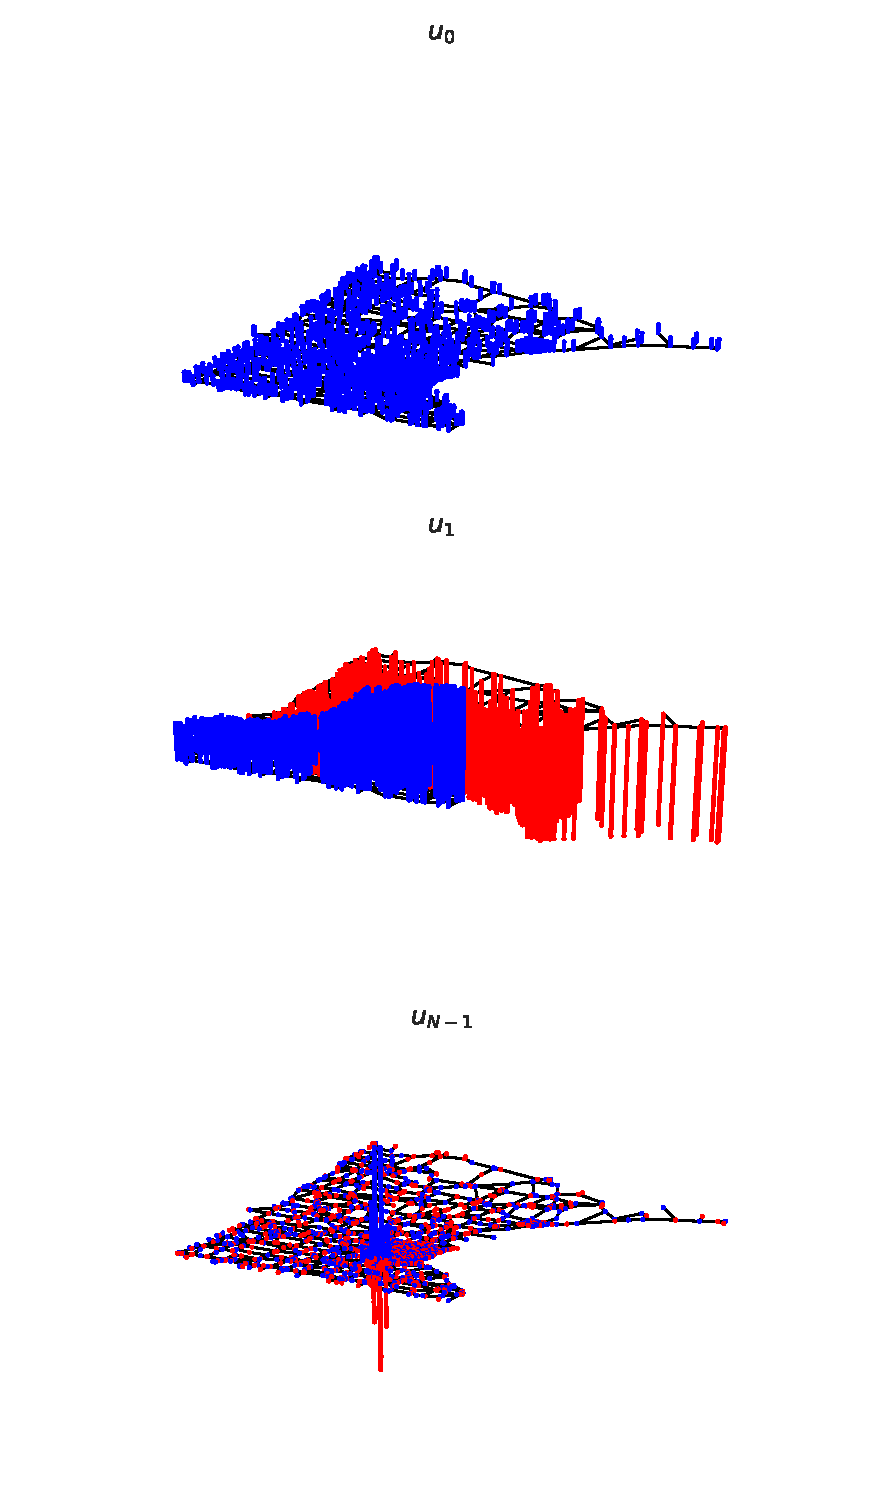
\includegraphics[trim={0 10cm 0 0},clip,width=\linewidth]{../img/graph_fourier_transform_5.pdf}
\end{figure}
  \end{column}
    \begin{column}{0.5\textwidth}
\begin{figure}
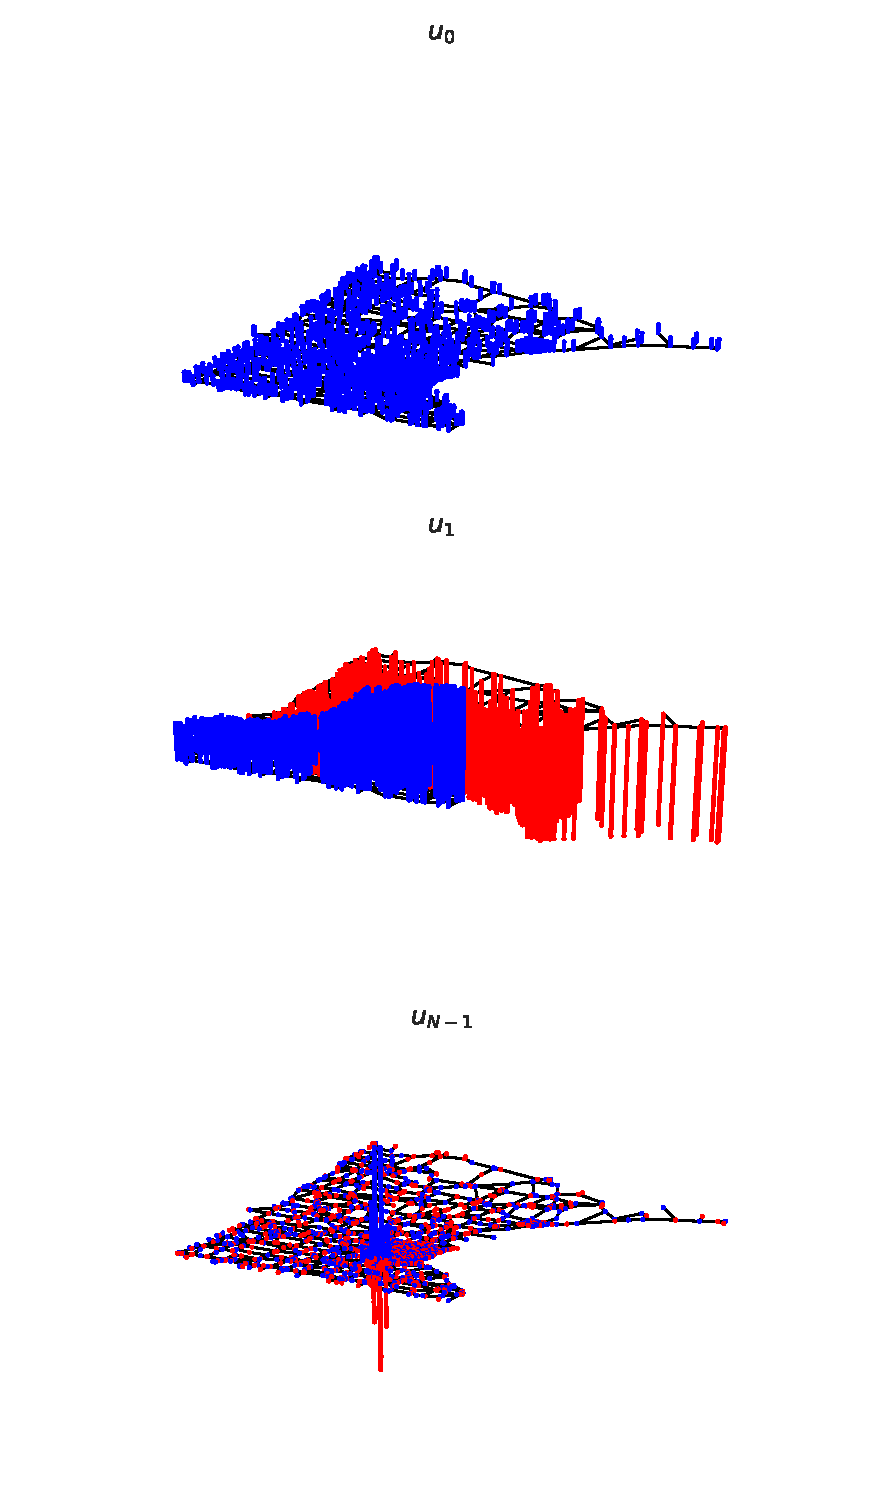
\includegraphics[trim={0 0 0 16cm},clip,width=\linewidth]{../img/graph_fourier_transform_5.pdf}
\end{figure}
  \end{column}
  \end{columns}
\end{frame}

\begin{frame}
  \frametitle{Fourier transform of a graph signal on a ring graph}
\begin{figure}
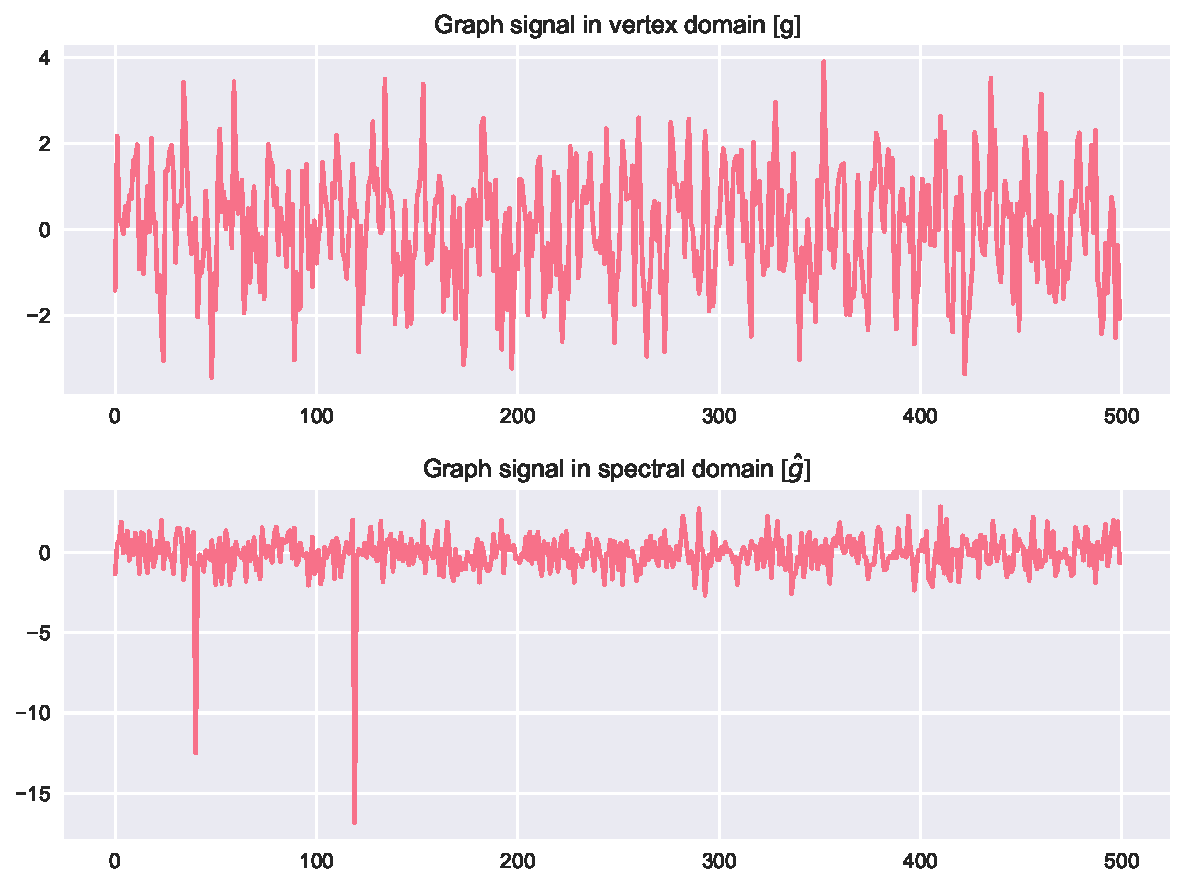
\includegraphics[width=0.7\linewidth]{../img/graph_fourier_transform_2.pdf}
\end{figure}
\end{frame}

\begin{frame}
  \frametitle{Signal smoothness depends on underlying structure of graph}
\begin{figure}
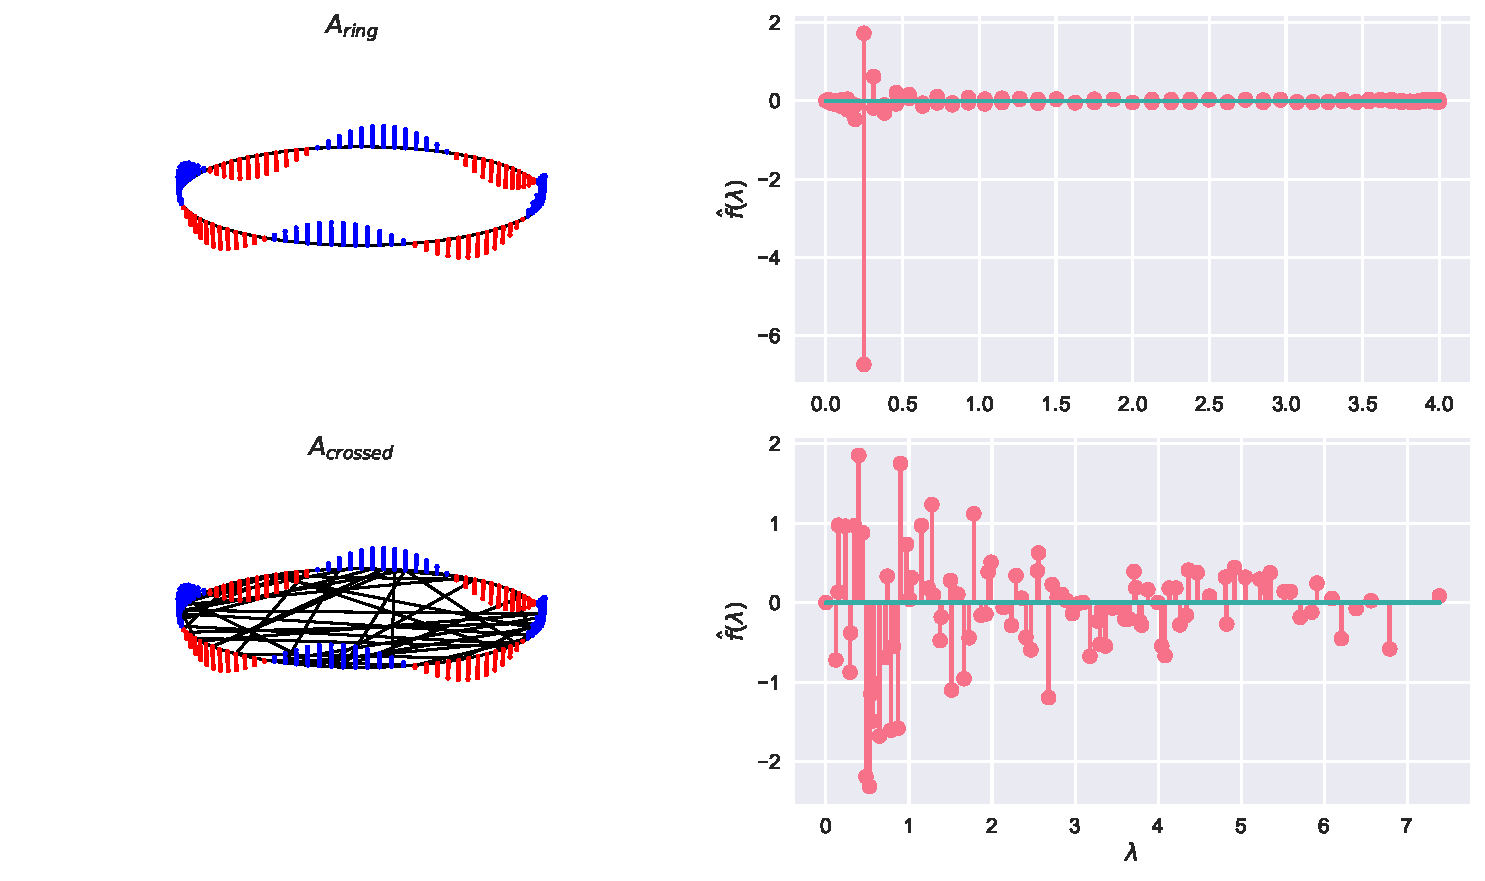
\includegraphics[width=0.9\linewidth]{../img/signal_smoothness_0.pdf}
\end{figure}
\end{frame}

\begin{frame}
  \frametitle{Measuring local signal smoothness on a graph}
  \begin{block}{The edge derivative of $f$ with respect to edge $e=(i,j)$}
    \begin{equation}
      \frac{\partial f}{\partial e} \bigg|_i = \sqrt{W_{i,j}} [f(j) - f(i)]
    \end{equation}
  \end{block}

  The local variation can be measured by the square root of the sum of the squared differences
  between signal values at adjacent vertices.
  
  \begin{block}{The local variation at vertex $i$}
    \begin{equation}
      || \nabla_i f || = \bigg[ \sum_{\text{e connected to i}} \bigg( \frac{\partial f}{\partial e} \bigg|_i \bigg)^2 \bigg]^{1/2} = \bigg[ \sum_{j \in N_i} W_{i,j} [f(j) - f(i)]^2 \bigg]^{1/2}
    \end{equation}
  \end{block}
\end{frame}

\begin{frame}
  \frametitle{Measuring global signal smoothness on a graph}

  \begin{block}{Discrete p-Dirichlet form of $f$}
    \begin{equation}
      S_p(f) = \frac{1}{p} \sum_{i \in V} \bigg[ \sum_{j \in N_i} W_{i,j} [f(j) - f(i)]^2 \bigg]^{\frac{p}{2}}
    \end{equation}
  \end{block}

  For $p=1$, $S_1$ is simply the sum of local variations across all vertices.

  For $p=2$, $S_2$ is a quadratic function of the Laplacian:

  \begin{block}{Graph Laplacian Quadratic Form}
    \begin{equation}
      \begin{split}
        S_2(f) = \frac{1}{2} \sum_{i \in V} \bigg[ \sum_{j \in N_i} W_{i,j}
        [f(j) - f(i)]^2 \bigg]^{\frac{1}{2}} = \sum_{(i, j) \in \epsilon}
        W_{i,j} [f(j) - f(i)]^2 \\
        = f^T L f
      \end{split}
    \end{equation}
  \end{block}

$S_2$ is small when $f$ has similar values at strongly-connected vertices.

\end{frame}


\begin{frame}
  \frametitle{Alternatives to the Graph Laplacian}

  \begin{block}{Normalized Graph Laplacian}
    \begin{equation}
      \tilde{L} = D^{-1/2} L D^{-1/2}
    \end{equation}
  \end{block}

  The eigenvalues of $\tilde{L}$ will be between 0 and 2. For bipartite graphs,
  the spectral folding phenomenon can be used.

  \begin{block}{Random Walk Matrix}
    \begin{equation}
      P = D^{-1} W
    \end{equation}
  \end{block}

  \begin{block}{Asymmetric Graph Laplacian}
    \begin{equation}
      L_a = I - D^{-1} W
    \end{equation}
  \end{block}
  
\end{frame}

\begin{frame}
  \frametitle{Filtering in the frequency/graph spectral domain}

  Using some transfer function $\hat{h}$, we can filter an input signal as follows:
  \begin{block}{Classical frequency filtering}
    \begin{equation}
      f_{out}(t) = \mathcal{F}^{-1} \{ \hat{f}_{in}(\xi) \hat{h}(\xi)\}
    \end{equation}
  \end{block}

  In the graph setting:
  
  \begin{block}{Graph filtering in the graph spectral domain}
    \begin{equation}
      \begin{split}
        \hat{h}(L) = U
        \begin{bmatrix}
          \hat{h}(\lambda_0) & & 0 \\
           & \ddots & \\
          0 & & \hat{h}(\lambda_{N-1})
        \end{bmatrix}
        U^*
      \\\\
      f_{out} = \hat{h}(L) f_{in}
      \end{split}
    \end{equation}
  \end{block}
  
\end{frame}

\begin{frame}
  \frametitle{Example: Gaussian Filtering}
  \begin{columns}
    \begin{column}{0.5\textwidth}
\begin{figure}
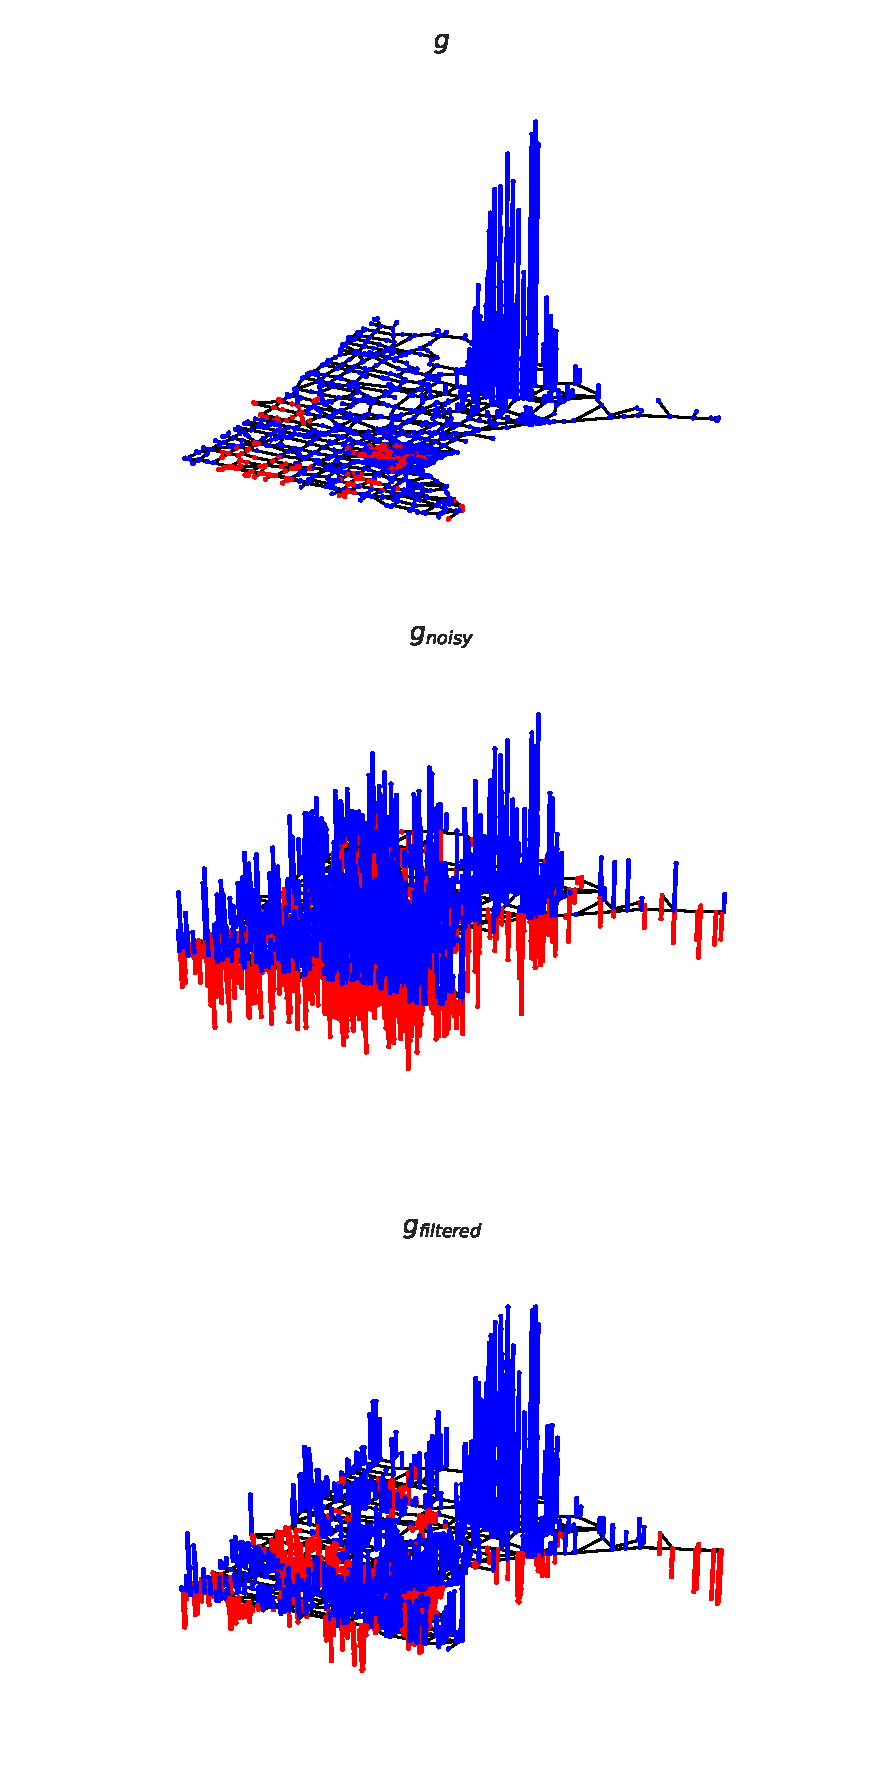
\includegraphics[trim={0 10cm 0 0},clip,width=\linewidth]{../img/basic_operations_1.pdf}
\end{figure}
  \end{column}
    \begin{column}{0.5\textwidth}
\begin{figure}
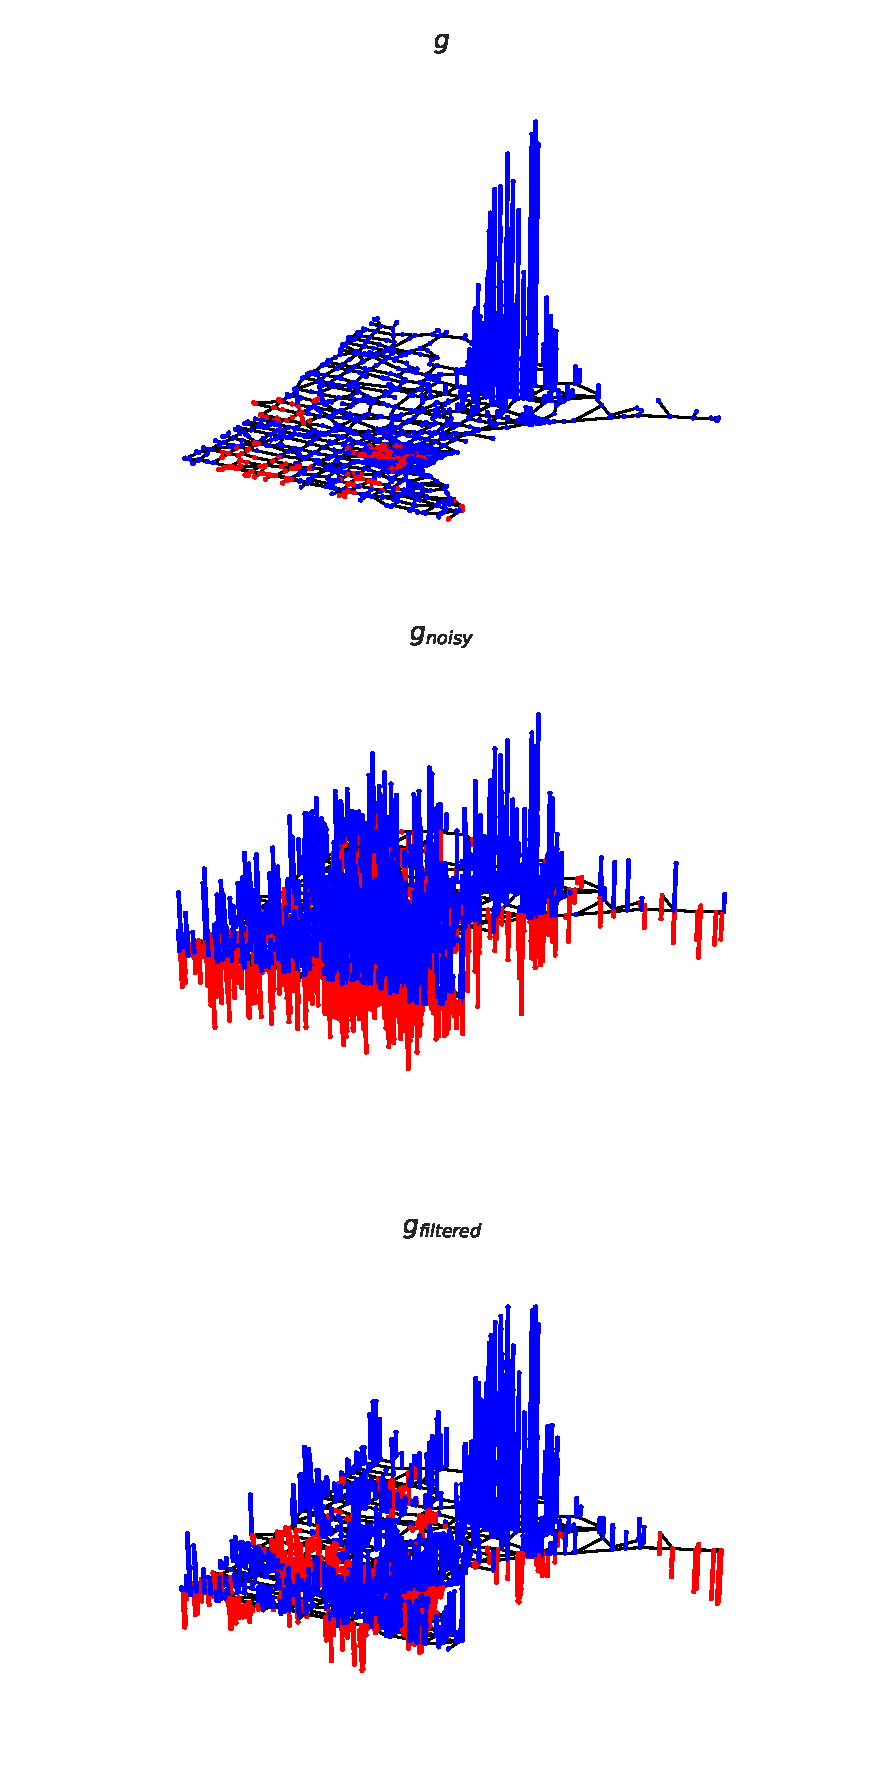
\includegraphics[trim={0 0 0 20cm},clip,width=\linewidth]{../img/basic_operations_1.pdf}
\end{figure}
  \end{column}
  \end{columns}
\end{frame}


\begin{frame}
  \frametitle{Filtering example: Tikhonov regularization}
\begin{figure}
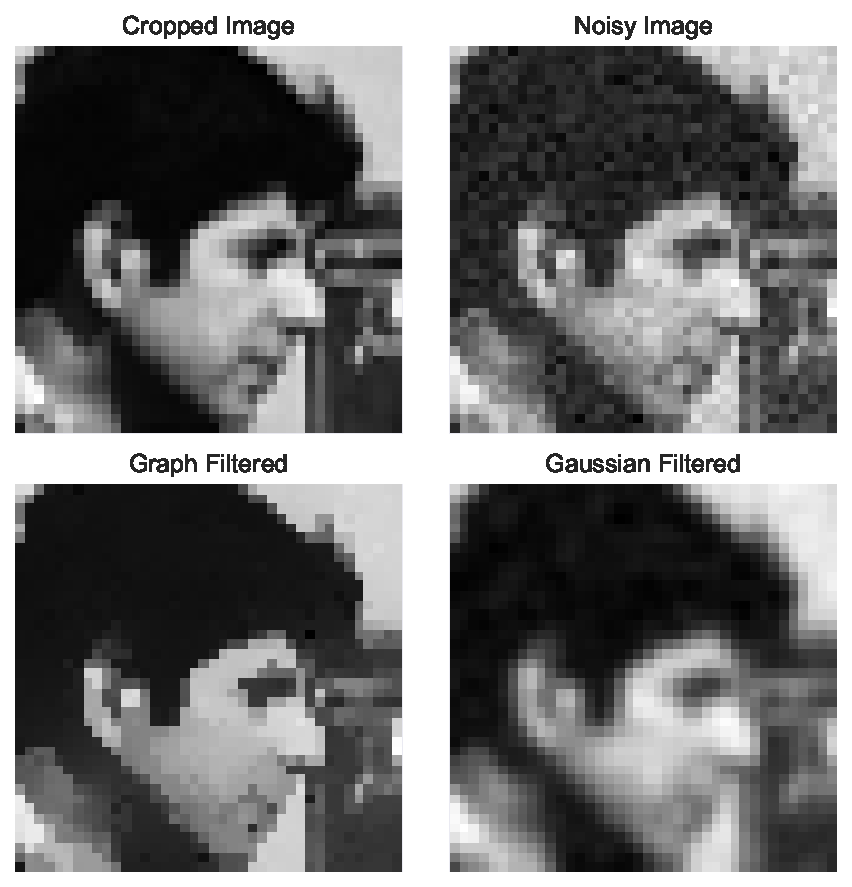
\includegraphics[width=0.5\linewidth]{../img/tikhonov_regularization_2.pdf}
\end{figure}
\end{frame}


\begin{frame}
  \frametitle{Filtering in the time/vertex domain}

  We can also filter in the time domain using convolution:

  \begin{block}{Classical time-domain filtering}
    \begin{equation}
      f_{out}(t) = (f_{in} * h)(t) 
    \end{equation}
  \end{block}

  In the graph setting, the output at any vertex $i$ is a linear combination of the elements of
  the input signal within a K-hop neighborhood (for some constants $b$):
  
  \begin{block}{Graph filtering in the vertex domain}
    \begin{equation}
      f_{out}(i) = b_{i,i} f_{in}(i) + \sum_{j \in N(i, K)} b_{i,j} f_{in}(j)
    \end{equation}
  \end{block}  
\end{frame}

\begin{frame}
  \frametitle{Equivalence of vertex/spectral filtering}
  If the frequency filter is a K-order polynomial $\hat{h} = \sum_{k=0}^K a_k
  \lambda_l^k$, the frequency filtered signal at vertex $i$ is a linear combination of the
  elements of the input signal at vertices within a K-hop neighborhood:

  \begin{block}{Frequency filtering when the filter is a K-order polynomial}
    \begin{equation}
      f_{out}(i) = b_{i,i} f_{in}(i) + \sum_{j \in N(i, K)} \sum_{d G(i,j)}^K a_k (L^k)_{i,j} f_{in}(j)
    \end{equation}
  \end{block}  
\end{frame}

\begin{frame}
  \frametitle{Convolution}

  Although we cannot directly generalize a convolution product on a graph
  because $h(t - \tau)$ is undefined, we can use frequency filtering, as
  previously defined:
  
  \begin{block}{Convolution of a signal on a graph}
    \begin{equation}
      (f * h)(i) = \sum_{l=0}^{N-1} \hat{f}(\lambda_l) \hat{h}(\lambda_l) u_l(i)
    \end{equation}
  \end{block}  
\end{frame}

\begin{frame}
  \frametitle{Translation}

  \begin{block}{Classical translation operation}
    \begin{equation}
      (T_vf)(t) = f(t - v) = (f * \delta_v)(t)
    \end{equation}
  \end{block}  

  Again, we cannot directly generalize $(t - v)$ for a graph, so we consider
  instead the definition of translation as convolution with a Dirac delta. 
  
  \begin{block}{Translation of a graph signal}
    \begin{equation}
     (T_n f)(i) = \sqrt{N} (f * \delta_n)(i) = \sqrt{N} \sum_{l=0}^{N-1} \hat{f}(\lambda_l) u_l^*(n) u_l(i)
    \end{equation}
  \end{block}  

Where:

\begin{equation}
  \delta_n =
  \begin{cases}
    1 \ if \ i=n \\
    0 \ otherwise
  \end{cases}
\end{equation}

\end{frame}

\begin{frame}
  \frametitle{Graph signal translation example}
  \begin{columns}
    \begin{column}{0.5\textwidth}
\begin{figure}
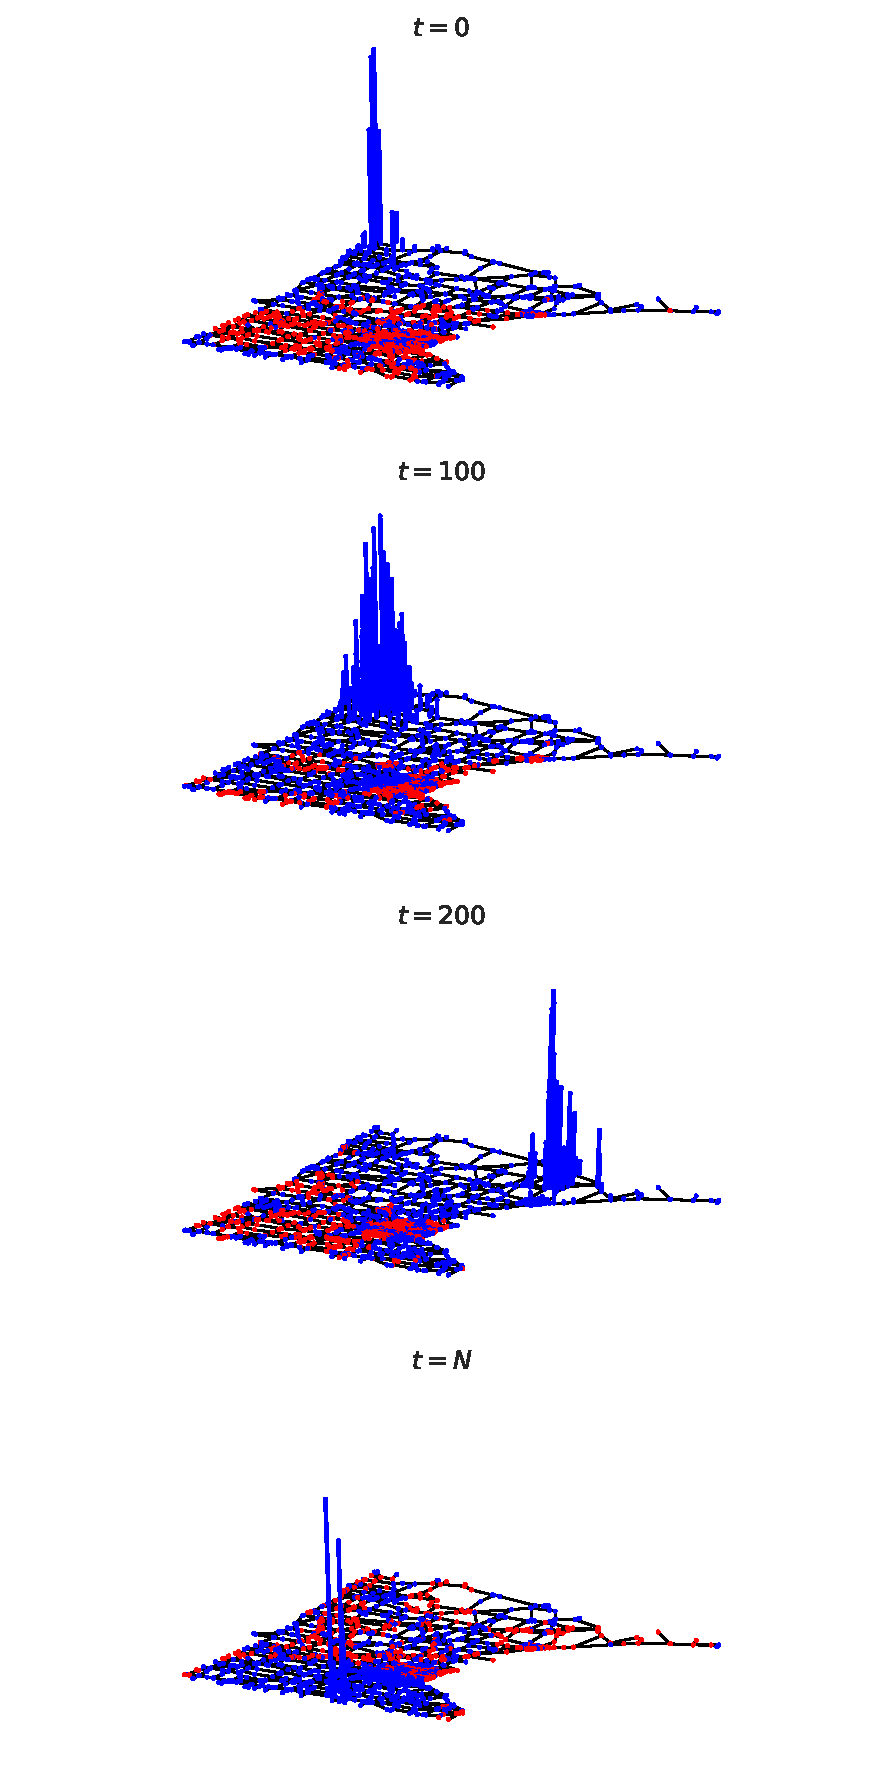
\includegraphics[trim={0 16cm 0 0},clip,width=\linewidth]{../img/basic_operations_0.pdf}
\end{figure}
  \end{column}
    \begin{column}{0.5\textwidth}
\begin{figure}
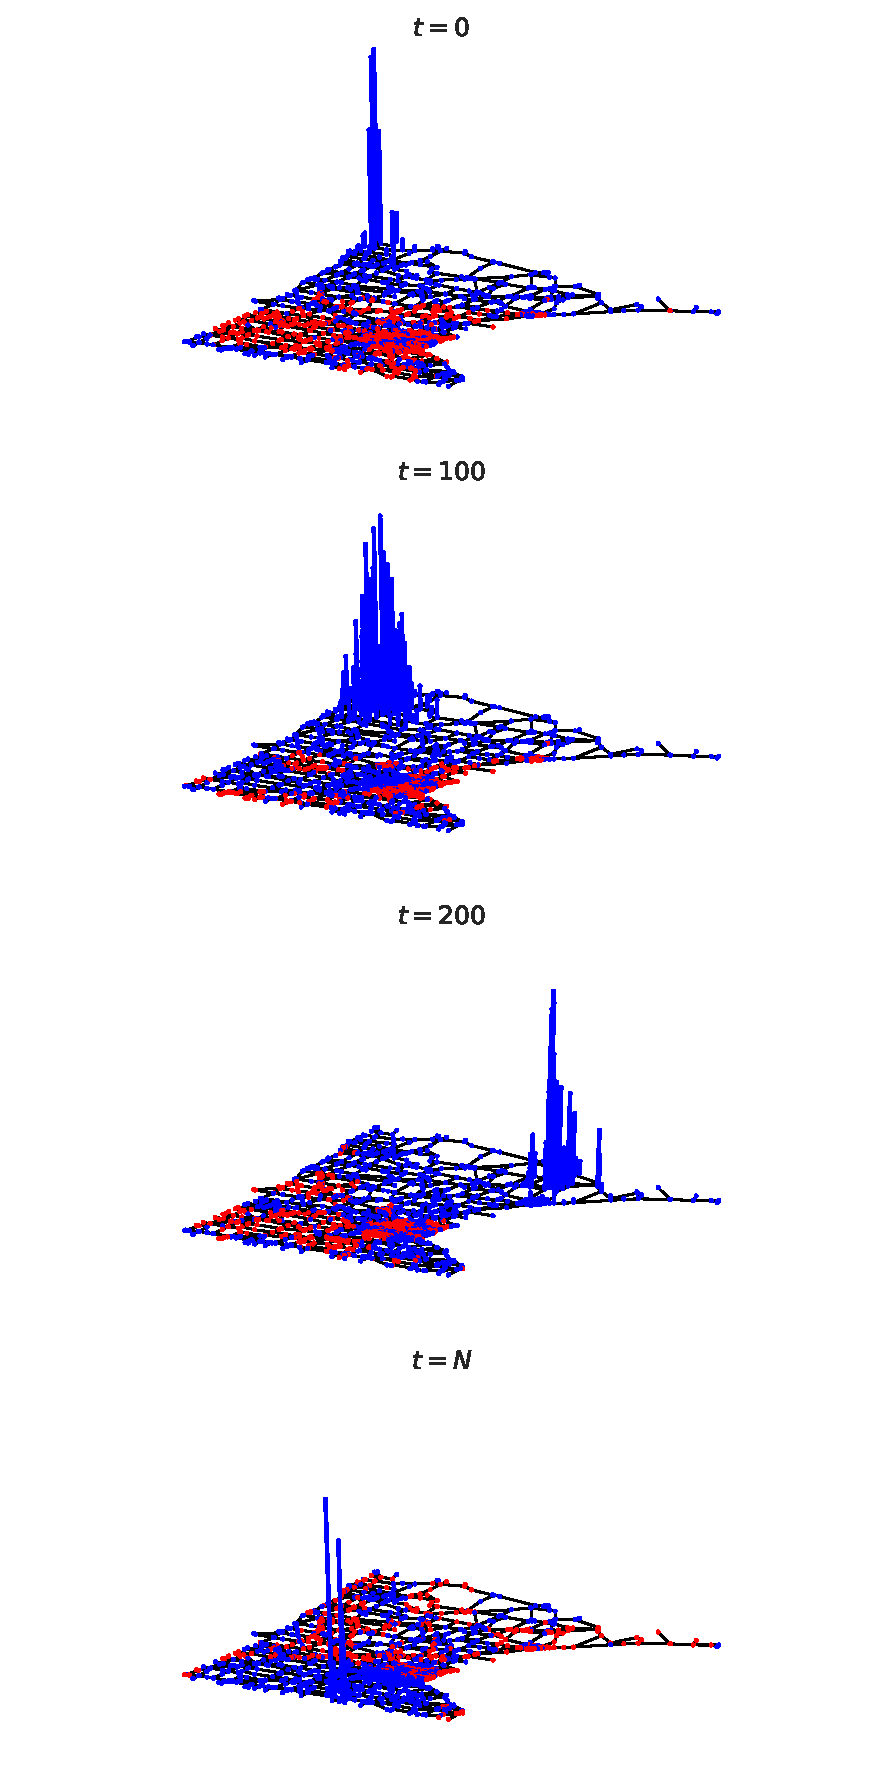
\includegraphics[trim={0 0 0 15cm},clip,width=\linewidth]{../img/basic_operations_0.pdf}
\end{figure}
  \end{column}
  \end{columns}
\end{frame}


\begin{frame}
  \frametitle{Modulation}

  In simple terms, like a ``translation'' in the frequency domain.
  
  \begin{block}{Classical modulation}
    \begin{equation}
      \begin{split}
        \text{Time domain: } (M_\omega f)(t) = e^{2 \pi j \omega t} f(t) \\
        \text{Frequency domain: } \overline{M_\omega f}(\xi) = \hat{f}(\xi -
        \omega)
      \end{split}
    \end{equation}
  \end{block}  

  Replace complex exponential with a graph Laplacian eigenvector:
  
  \begin{block}{Graph modulation}
    \begin{equation}
      (M_kf)(i) = \sqrt{N} u_k(i) f(i)
    \end{equation}
  \end{block}  

  If a kernel $f$ is localized around 0 in the graph spectral domain, then
  $\overline{M_kg}$ is localized around $\lambda_k$.
\end{frame}

\begin{frame}
  \frametitle{Graph signal modulation example}
  \begin{columns}
    \begin{column}{0.5\textwidth}
\begin{figure}
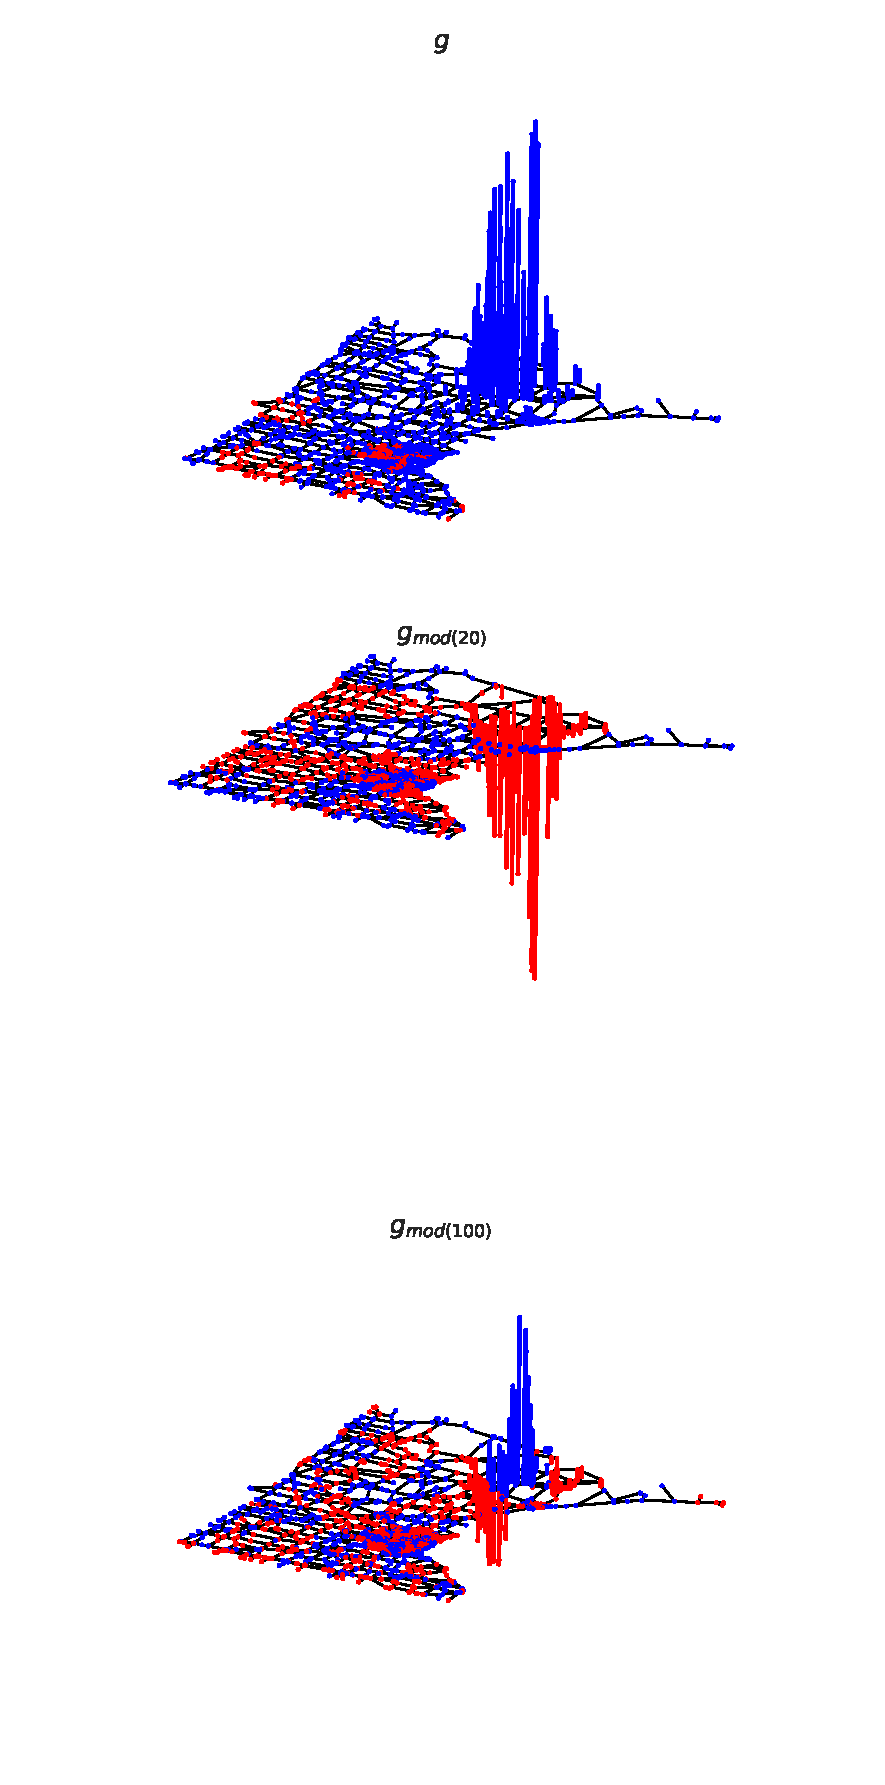
\includegraphics[trim={0 10cm 0 0},clip,width=\linewidth]{../img/basic_operations_3.pdf}
\end{figure}
  \end{column}
    \begin{column}{0.5\textwidth}
\begin{figure}
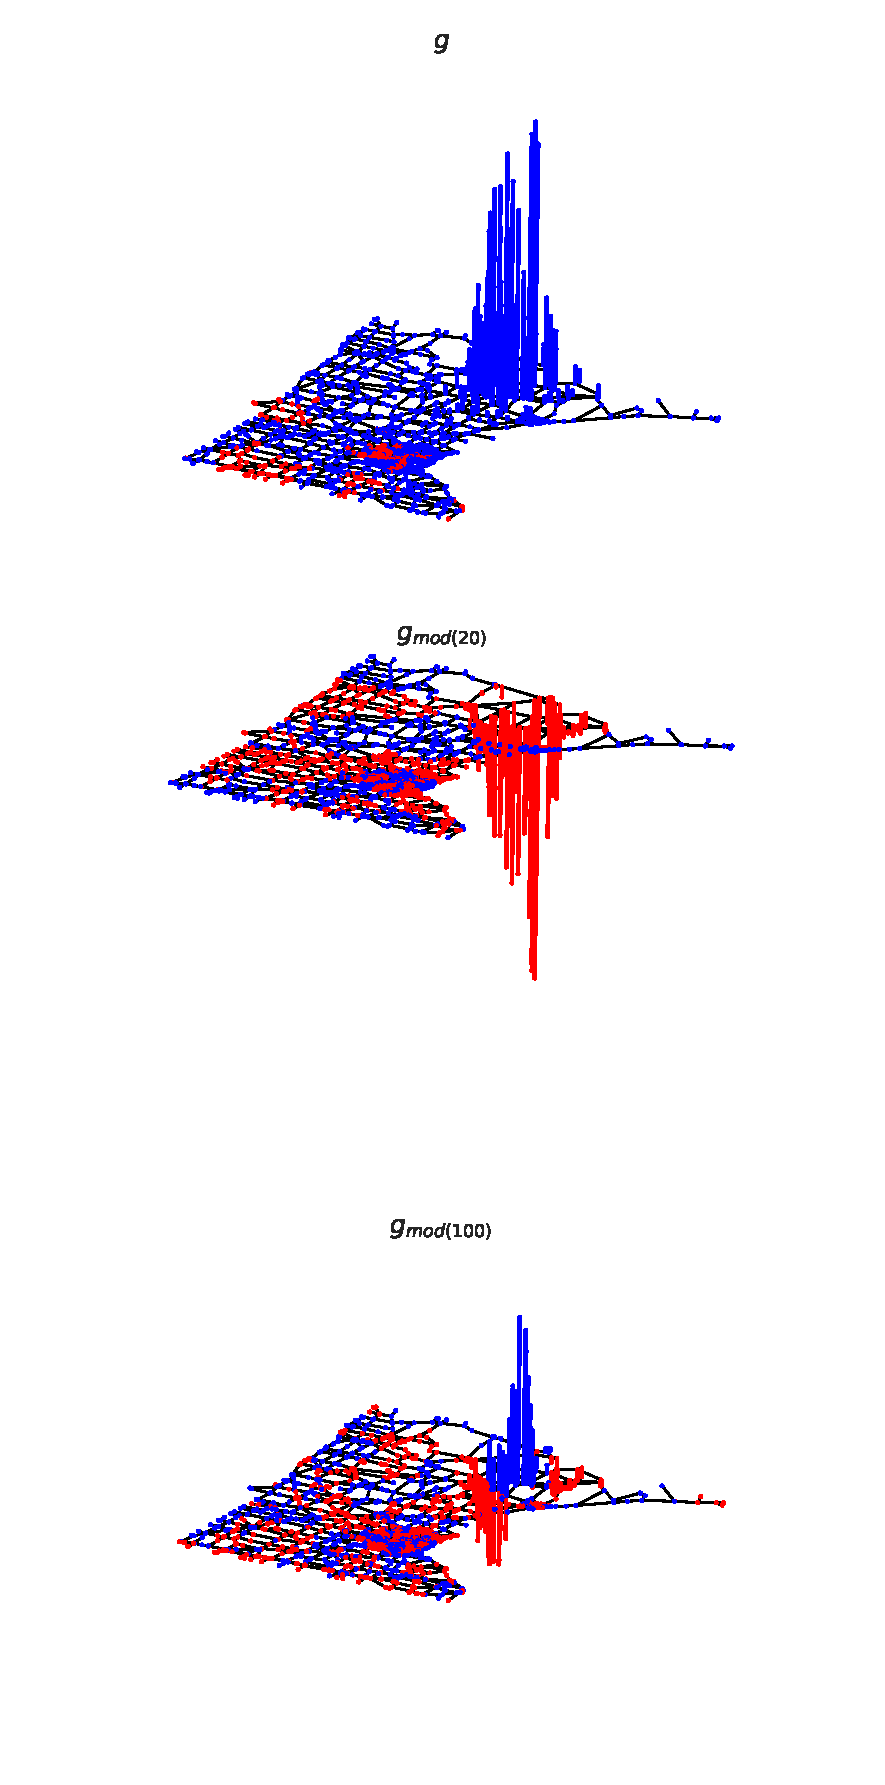
\includegraphics[trim={0 0 0 20cm},clip,width=\linewidth]{../img/basic_operations_3.pdf}
\end{figure}
  \end{column}
  \end{columns}
\end{frame}


\begin{frame}
  \frametitle{Dilation}

  \begin{block}{Classical dilation}
    \begin{equation}
      \begin{split}
        \text{Time domain: } (D_s f)(t) = \frac{1}{s} f \bigg( \frac{t}{s} \bigg) \\
        \text{Frequency domain: } \overline{D_s f}(\xi) = \hat{f}(s \xi)
      \end{split}
    \end{equation}
  \end{block}  

  Replace the frequency $\xi$ with an eigenvalue of the Laplacian.
  
  \begin{block}{Graph dilation}
    \begin{equation}
      (D_sf)(\lambda) = \hat{f} (s \lambda)
    \end{equation}
  \end{block}  
\end{frame}

\begin{frame}
  \frametitle{Graph signal dilation example}
  \begin{columns}
    \begin{column}{0.5\textwidth}
\begin{figure}
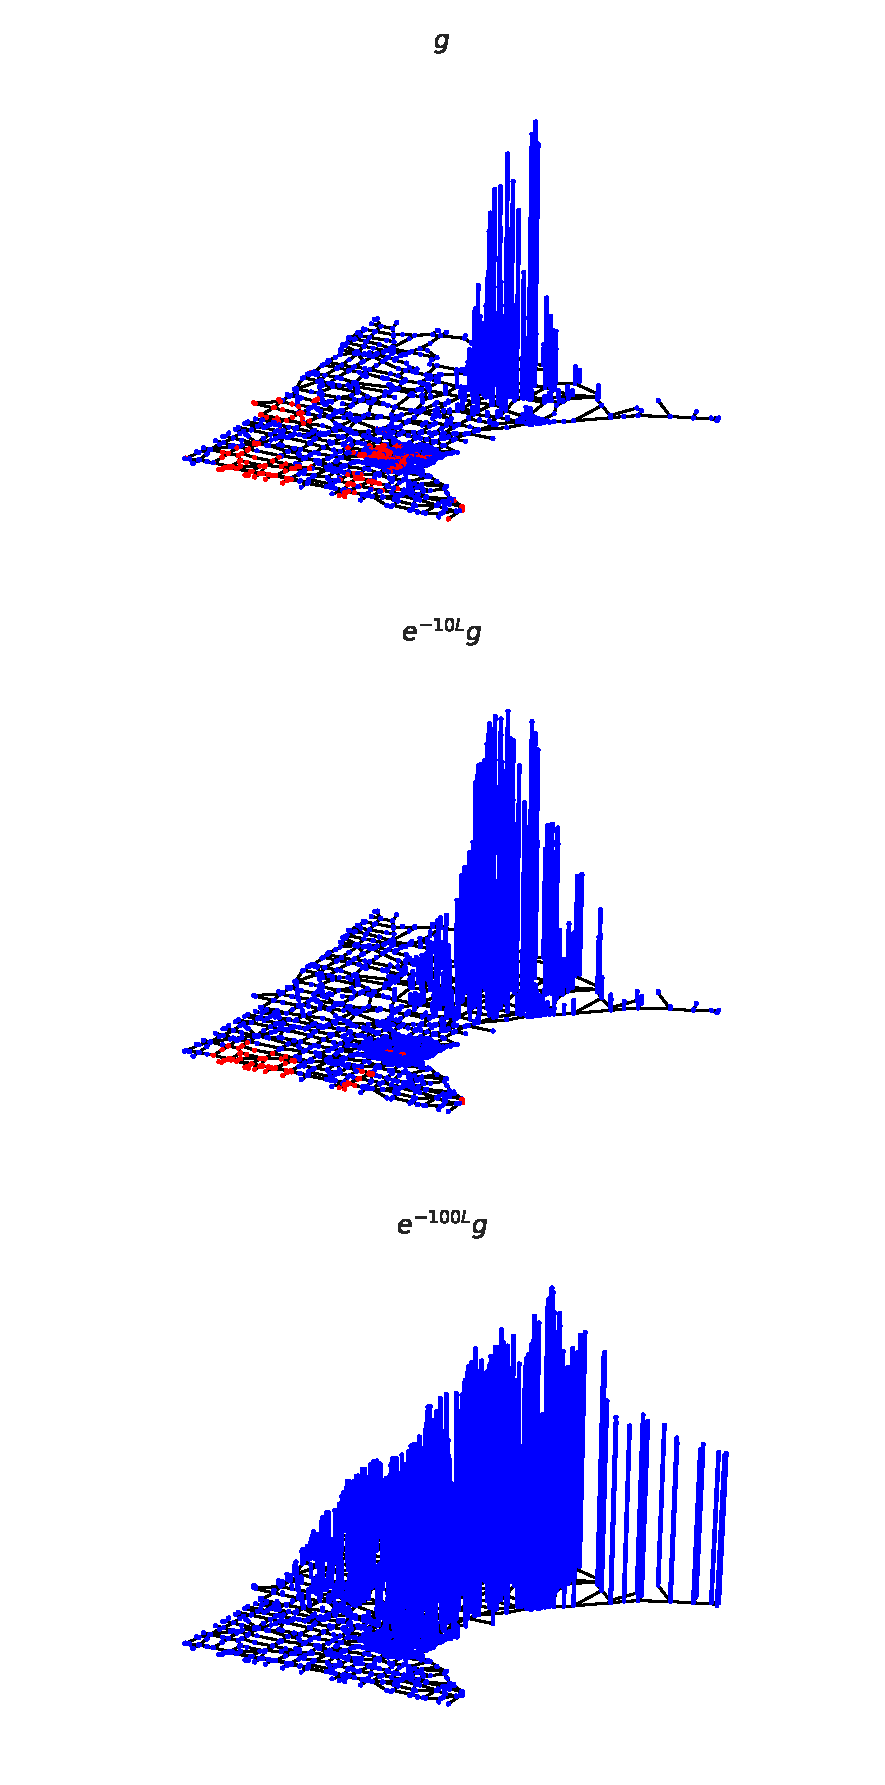
\includegraphics[trim={0 10cm 0 0},clip,width=0.9\linewidth]{../img/basic_operations_4.pdf}
\end{figure}
  \end{column}
    \begin{column}{0.5\textwidth}
\begin{figure}
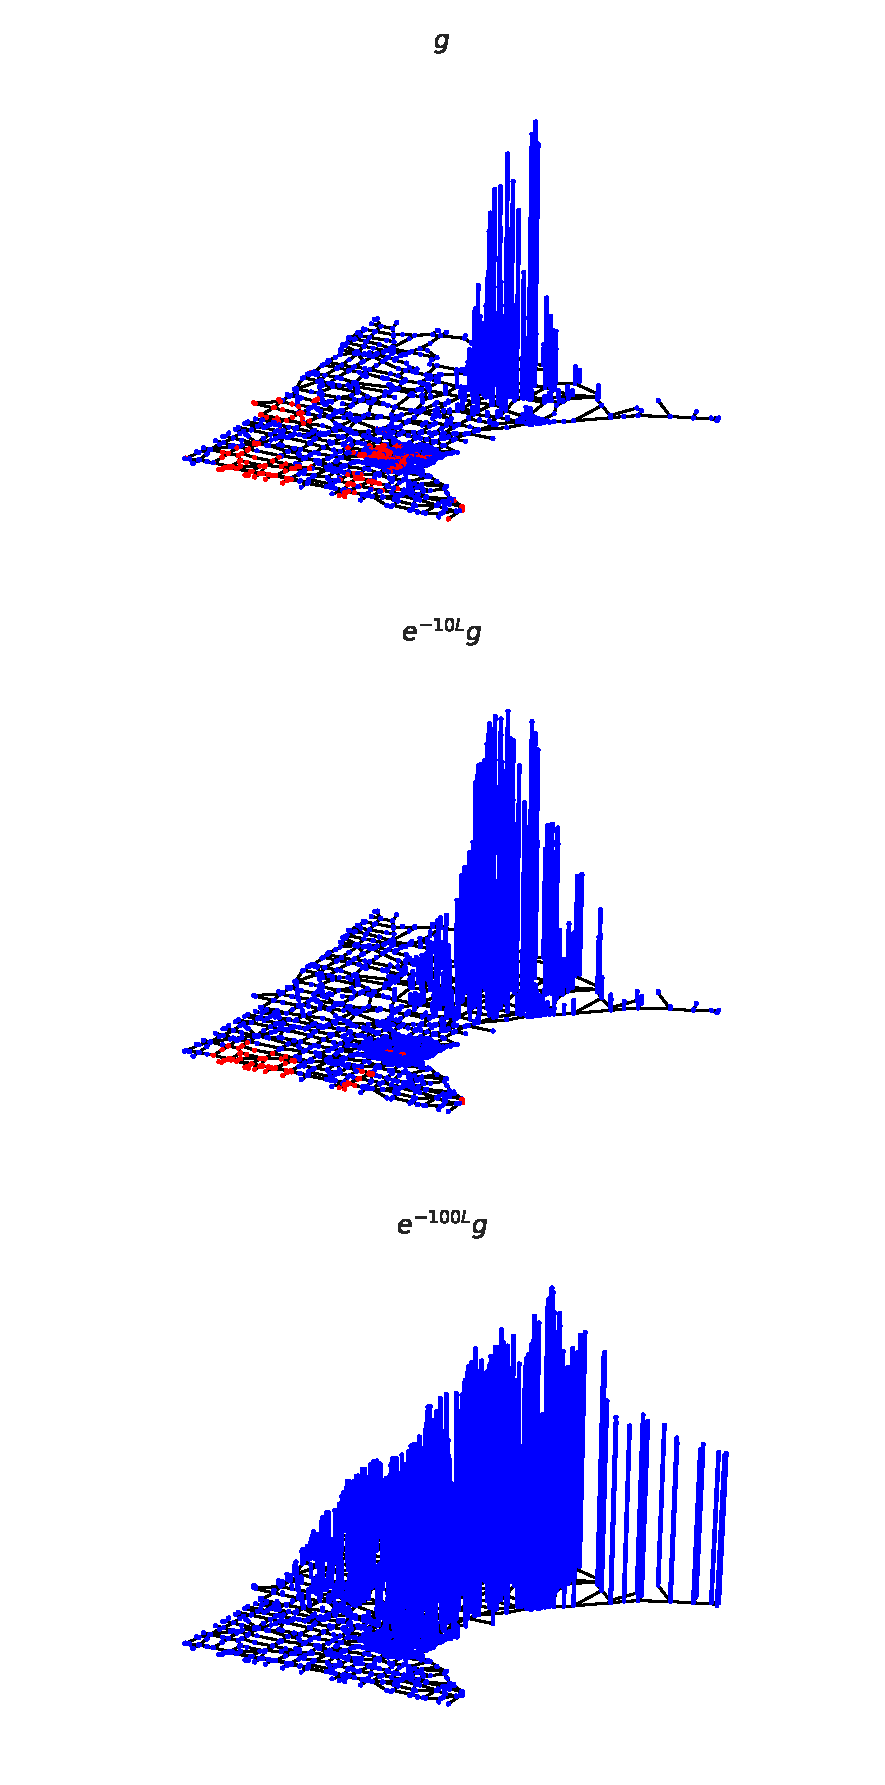
\includegraphics[trim={0 0 0 20cm},clip,width=0.9\linewidth]{../img/basic_operations_4.pdf}
\end{figure}
  \end{column}
  \end{columns}
\end{frame}


\begin{frame}
  \frametitle{Graph coarsening, downsampling and reduction}

  \begin{itemize}
  \item For bipartite graphs, one can recursively downsample by a factor of two
  \item Downsampling based on diffusion distances
  \item Greedy seed selection algorithm
  \item Recursive spectral bisection
  \item Minimize number of edges connecting two vertices in a downsampled subset
  \end{itemize}
\end{frame}

\begin{frame}
  \frametitle{Example: Spectral clustering}
\begin{figure}
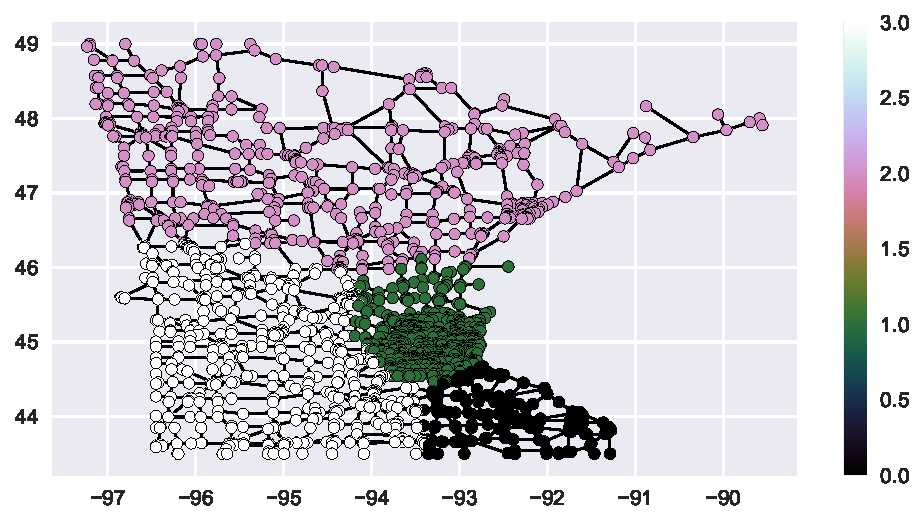
\includegraphics[trim={1cm 0.7cm 2cm 0},clip,width=0.9\linewidth]{../img/clustering_methods_1.pdf}
\end{figure}
\end{frame}

\begin{frame}
  \frametitle{Example: Recursive spectral bisection}
\begin{figure}
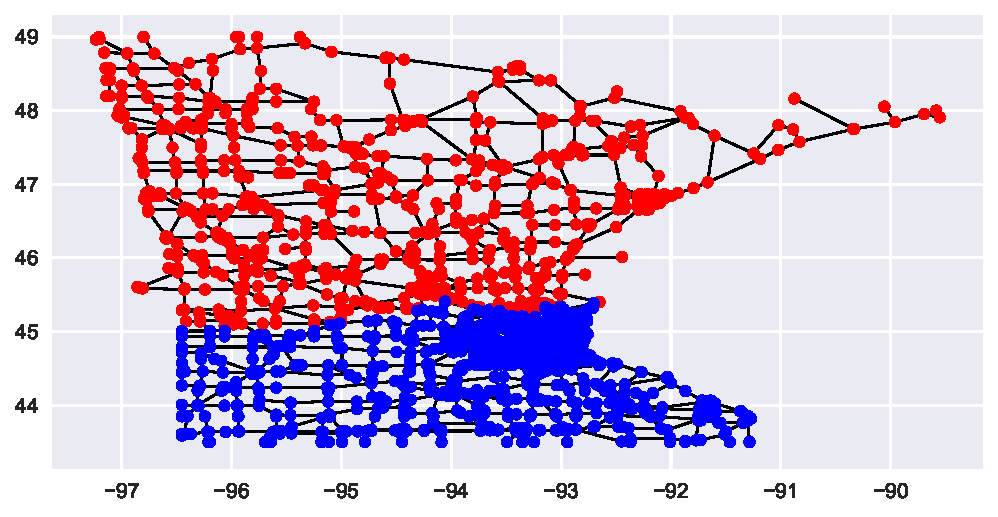
\includegraphics[trim={1cm 0.7cm 0 0},clip,width=0.5\linewidth]{../img/clustering_methods_2.pdf}
\end{figure}
\begin{figure}
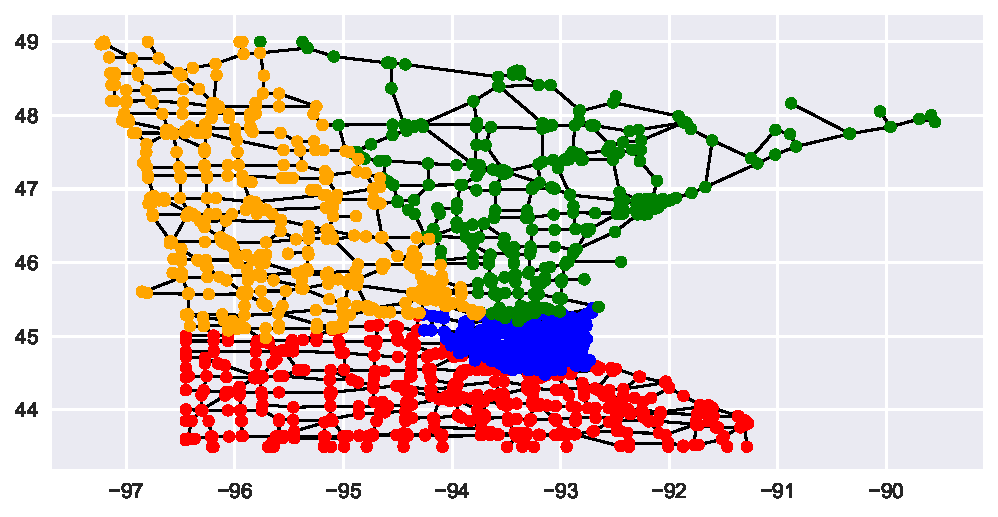
\includegraphics[trim={1cm 0.7cm 0 0},clip,width=0.5\linewidth]{../img/clustering_methods_3.pdf}
\end{figure}
\end{frame}


\begin{frame}
  \frametitle{Localized multiscale transforms}

  Measuring the spread of graph signals in both time and frequency domains:

  \begin{block}{Spatial spread of a signal f around a center vertex i}
    \begin{equation}
      \Delta_{G,i}^2(f) = \frac{1}{|| f ||_2^2} \sum_{j \in V} [d_G(i, j)]^2 [f(j)]^2
    \end{equation}
  \end{block}  

  \begin{itemize}
  \item Where $d_G(i, \cdot)$ is the geodesic distance function.
  \item $[f(j)]^2 / || f ||^2$ represents the pmf of signal $f$.
  \item $\Delta_{G, i}^2$ is the variance of the geodesic distance function at
    node i.
  \end{itemize}
\end{frame}

\begin{frame}
  \frametitle{Localized multiscale transforms}
  
  The spatial and spectral spreads can thus both be characterized:

  \begin{block}{Total spatial spread of a graph signal}
    \begin{equation}
      \Delta_{G}^2(f) = min_{i \in V} \{ \Delta_{G, i} (f) \}
    \end{equation}
  \end{block}  
  \begin{block}{Total spectral spread of a graph signal}
    \begin{equation}
      \Delta_{\sigma}^2(f) = min_{\mu \in \mathcal{R}} \bigg\{ \frac{1}{|| f ||_2^2} \sum_{\lambda \in \sigma(L)} [\sqrt{\lambda} - \sqrt{\mu}]^2 [\hat{f}(\lambda)]^2 \bigg\}
    \end{equation}
  \end{block}  
 \end{frame} 
  
 \begin{frame}
   \frametitle{Wavelets in the vertex domain}
    The wavelet function $\Psi$ at scale k and center vertex i is defined by:

  \begin{block}{Wavelet in the vertex domain around a vertex i}
  \begin{equation}
  \Psi_{k,i}^{CKWT} (j) = \frac{a_{k, \tau}}{|\partial N_{(i, \tau)}|}, \forall j \in \partial N(i, \tau)
  \end{equation}
  \end{block}

  Where $\partial N_{(i, \tau)}$ is the set of all vertices $j \in N$ such that the geodesic distance between $i$ and $j$ is $\tau$. $a_{k, \tau}$ is a set of coefficients that approximate the continuous wavelet function. 

  \begin{block}{Wavelet Transform}
  \begin{equation}
  \mathbf{\Psi}_{k}^{CKWT} = [\Psi_{k,1}^{CKWT} ; \Psi_{k,2}^{CKWT} \cdots \Psi_{k,N}^{CKWT}]
  \end{equation}
  \end{block}
 
 \end{frame}
 
\begin{frame}
  \frametitle{Example: Ricker wavelet}
\begin{figure}
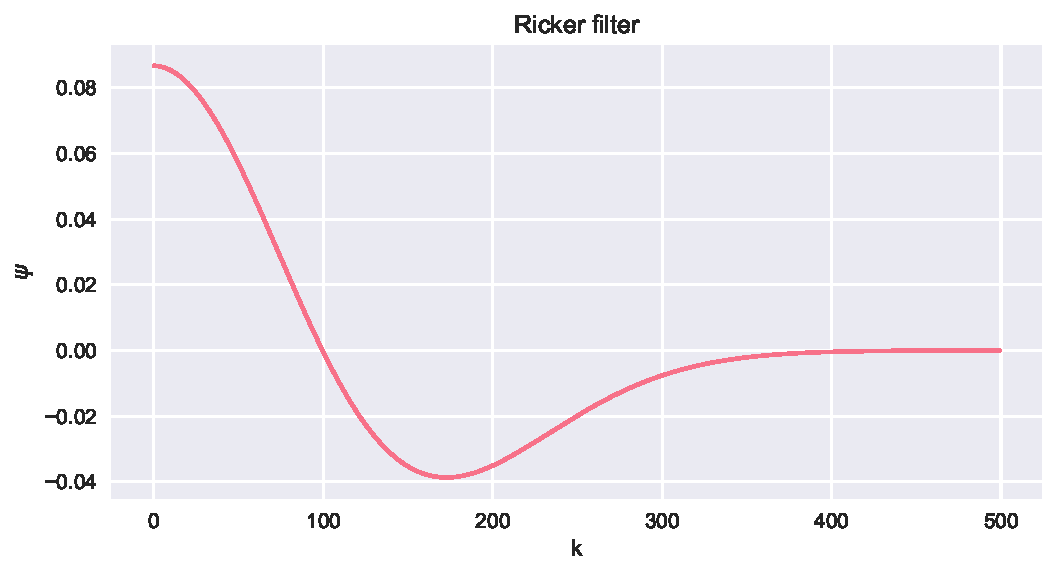
\includegraphics[width=0.9\linewidth]{../img/wavelet_filter_0.pdf}
\end{figure}
\end{frame}

\begin{frame}
  \frametitle{Example: Applying Ricker Wavelet Transform for edge detection}
\begin{figure}
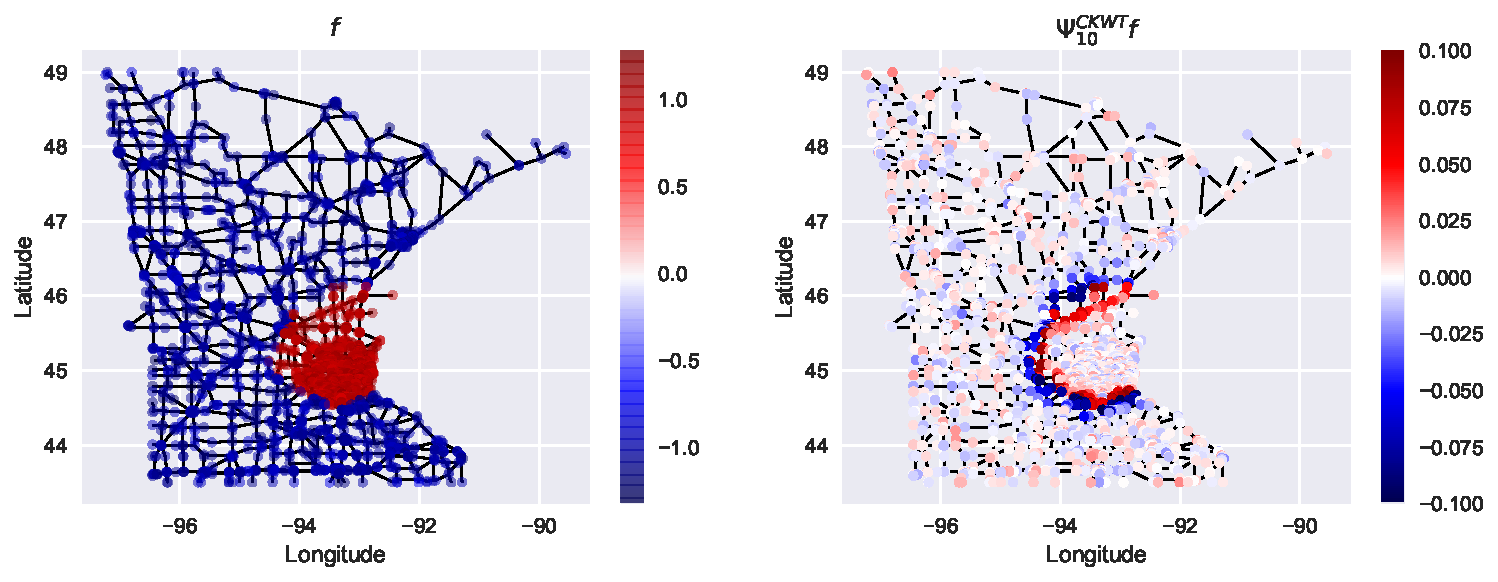
\includegraphics[width=0.9\linewidth]{../img/wavelet_filter_1.pdf}
\end{figure}
\end{frame}

\begin{frame}
  \frametitle{Example: Tradeoff between spectral and spatial spread}
\begin{figure}
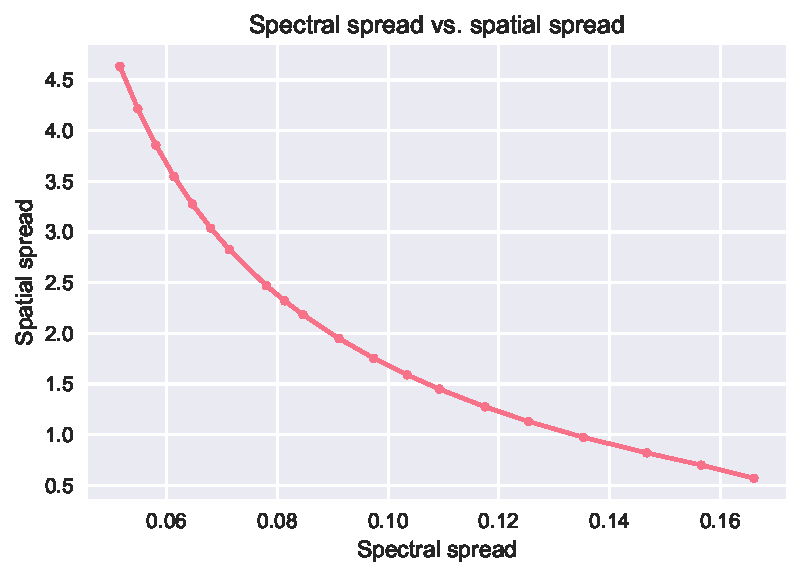
\includegraphics[width=0.9\linewidth]{../img/wavelet_filter_7.pdf}
\end{figure}
\end{frame}
 
\section{Strengths and weaknesses}

\begin{frame}
  \frametitle{Strengths and weaknesses}
  Strengths:

  \begin{itemize}
  \item Highly accessible
  \item Comprehensive introduction to signal processing on graphs
  \item Excellent examples and illustrations from different fields
  \end{itemize}

  Weaknesses:

  \begin{itemize}
  \item Doesn't emphasize computational difficulty of several proposed methods
  \item Some notation could be simplified
  \item Some assertions aren't proved or expanded upon
  \item Couldn't find any code
  \end{itemize}
\end{frame}
\section{Extensions and applications}

\begin{frame}
  \frametitle{Extensions and applications}
  \begin{itemize}
    \item Little is known about how the structure of the graph affects transforms
    \item Unclear when to use different graph matrices (Laplacian, Normalized
      Laplacian, etc.)
    \item Unclear when to use different distance metrics (geodesic, algebraic,
      diffusion, resistance, etc.)
    \item Computing the eigendecomposition of the Laplacian is \textbf{slow}
  \end{itemize}
\end{frame}


\begin{frame}
\frametitle{Appendix}

For an infinite square lattice grid, it can be shown that the Graph Laplacian
corresponds to the continuous Laplacian as $\epsilon \rightarrow 0$:

  \begin{block}{Equivalence between Continous and Graph Laplacians}
    \begin{equation}
      \frac{\partial^2 F}{\partial x^2} = \lim_{\epsilon \rightarrow 0} \frac{[F(x + \epsilon) - F(x)] + [F(x - \epsilon) - F(x)]}{\epsilon^2}
    \end{equation}
  \end{block}

\end{frame}

\end{document} 